\documentclass[border={0pt 0pt 0pt 0pt},convert={density=300,outext=.png}]{standalone}

\usepackage{tikz}
\usepackage{pgf}
\usepackage{subcaption}
% \usepackage[margin=0.5pt]{geometry}
\usetikzlibrary{calc}   % coordinate calculation

\newcommand{\defstuff} {
  \def \step {1}
  \def \cc {\step/2}  % center of cell
  \coordinate (offset) at ($(\cc,\cc)$);
}

\newcommand{\drawgrid}[1] {
  \draw[step=\step, color=gray] (0,0) grid ($#1$); % draw the grid, base at #1
}

\newcommand{\drawrobots}[1] {
    \foreach \coord in #1 {
      \coordinate[at=\coord, name=A];
      \draw ($(A) + (offset)$) circle ({\cc*0.8});
    }
}

\newcommand{\drawarrows}[1] {
    \foreach \a/\b in #1 {
      \coordinate[at=\a, name=A];
      \coordinate[at=\b, name=B];
      \draw[->, color=darkgray] ($(A) + (offset)$) -- ($(B) + (offset)$);
    }
}

\newcommand{\spacee}[3] {
  \begin{tikzpicture}[thick, scale=0.6]
    \defstuff
    \drawgrid{#1}
    \drawrobots{#2}
    \drawarrows{#3}
  \end{tikzpicture}
}


\begin{document}

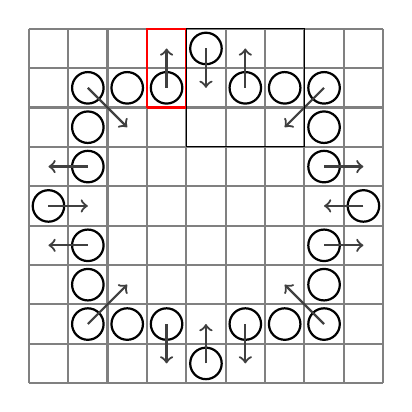
\begin{tikzpicture}[thick,scale=0.5]
  \defstuff
  \drawgrid{(9,9)}
\drawrobots{{(7, 3), (5, 7), (4, 8), (7, 7), (2, 1), (1, 3), (1, 6), (5,
    1), (3, 7), (7, 2), (4, 0), (1, 2), (6, 7), (7, 6), (1, 5), (0, 4), (1,
      1), (7, 1), (7, 5), (2, 7), (6, 1), (3, 1), (1, 7), (8, 4)}}
  \drawarrows{{{(1, 5)/(0, 5)},{(5, 7)/(5, 8)},{(5, 1)/(5, 0)},{(0, 4)/(1,
      4)},{(7, 7)/(6, 6)},{(7, 1)/(6, 2)},{(3, 1)/(3, 0)},{(1, 1)/(2, 2)},{(1,
        3)/(0, 3)},{(1, 7)/(2, 6)},{(8, 4)/(7, 4)},{(7, 5)/(8, 5)},{(4, 8)/(4,
          7)},{(7, 3)/(8, 3)},{(3, 7)/(3, 8)},{(4, 0)/(4, 1)}}}
  \draw[thick,red] (3,7) -- (4,7) -- (4,9) -- (3,9) -- (3,7);
  \draw[thin] (4,6) -- (7,6) -- (7,9) -- (4,9) -- (4,6);
\end{tikzpicture}


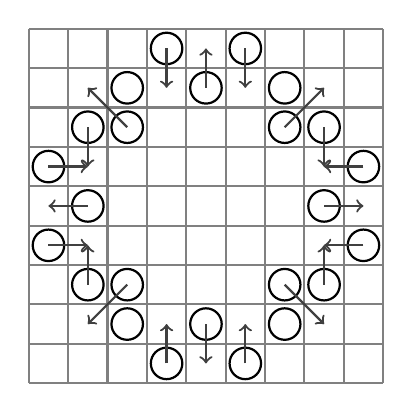
\begin{tikzpicture}[thick,scale=0.5]
  \defstuff
  \drawgrid{(9,9)}
  \drawrobots{{(4, 7), (6, 6), (3, 0), (2, 1), (6, 2), (1, 6), (0, 3),
  (8, 5), (7, 2), (1, 2), (7, 4), (6, 7), (7, 6), (5, 8), (5, 0), (2, 2),
  (4, 1), (2, 6), (1, 4), (0, 5), (2, 7), (8, 3), (6, 1), (3, 8)}}
  \drawarrows{{{(3,
  8)/(3, 7)},{(1, 2)/(1, 3)},{(0, 3)/(1, 3)},{(7, 2)/(7, 3)},{(7, 4)/(8,
  4)},{(3, 0)/(3, 1)},{(7, 6)/(7, 5)},{(2, 2)/(1, 1)},{(5,
  8)/(5, 7)},{(2, 6)/(1, 7)},{(1, 4)/(0, 4)},{(6, 2)/(7,
  1)},{(6, 6)/(7, 7)},{(4, 7)/(4, 8)},{(5, 0)/(5, 1)},{(0,
  5)/(1, 5)},{(4, 1)/(4, 0)},{(1, 6)/(1, 5)},{(8, 5)/(7, 5)},{(8, 3)/(7,
  3)}}}
\end{tikzpicture}

\end{document}
